\documentclass[12pt,fleqn]{article}\usepackage{../../common}
\begin{document}
Sinyaller, Geriye Dönük Analiz, Performans

Elimizde bir zaman serisi var, bu seri bir finansal varlığın fiyat seviyesi
olabilir, belki bir tahvildir, belki altın fiyatıdır, ilk gün 100 ikinci gün 102
olmuş, böyle gidiyor.

\begin{minted}[fontsize=\footnotesize]{python}
d = np.array([100,102,104.04,106.12,108.24,110.41])
\end{minted}

Peki bu fiyat seviyeleri günlük hangi yüzde değişimlerine tekabül ediyor?  Bu
hesabın \verb!pandas! ile kolay bir yolu var, \verb!pct_change! kullanabiliriz,

\begin{minted}[fontsize=\footnotesize]{python}
import pandas as pd
p = pd.Series(d)
print (list(np.round(p.pct_change(),2)))
\end{minted}

\begin{verbatim}
[nan, 0.02, 0.02, 0.02, 0.02, 0.02]
\end{verbatim}

Her gün yüzde 2'lik bir değişim varmış (bu yazı için veri uydururken fiyat
seviyelerini ona göre ayarladık).

Şimdi sadece yüzde değişimleri ve başlangıç fiyat seviyesini kullanarak seriyi
tekrar üretebilir miydik? Tek yüzde değişimle bir sonraki sayıyı nasıl elde
ederiz?  Mesela 100'den yüzde 2 değişimle sonraki değere geçeceğiz, kolay, 1
artı 0.02 yani 1.02 değerini 100 ile çarparız, sonraki sayı çıkar, 102. Bu
metotu diğer yüzde değişimler için kullanabiliriz. O zaman tüm fiyat
seviyelerini hesap için eldeki yüzde değişim listesine 1 sayısını eklersek,
1.02, 1.02, .. elde edilir, ve bu rakamları başta 100 ile, sonra birbirleri ile
çarparsak tüm fiyat listesini tekrar elde ederiz. Bir dizinin tüm öğelerinin
birer birer çarpılıp bunun kümülatif olarak gösterilmesini \verb!cumprod!
halleder,

\begin{minted}[fontsize=\footnotesize]{python}
ret = p.pct_change()
100*np.cumprod(1+ret)
\end{minted}

\begin{verbatim}
Out[1]: 
0       NaN
1    102.00
2    104.04
3    106.12
4    108.24
5    110.41
dtype: float64
\end{verbatim}

Üstteki hesabı bir al-tut stratejisinin performansı olarak ta görebiliriz bu
durumda illa baştaki 100 değerini kullanmaya gerek yok, 100 yerine 1 dersek o
zaman bu stratejiye koyulmuş 1 liranın, 1 doların ne kadar büyüyeceğini görmüş
oluruz.  1 lira 2 lira olduysa mesela bu ikiye katlama demektir, performansın
iyi olduğu sonucuna varabiliriz.

\begin{minted}[fontsize=\footnotesize]{python}
1*np.cumprod(1+ret)
\end{minted}

\begin{verbatim}
Out[1]: 
0       NaN
1    1.0200
2    1.0404
3    1.0612
4    1.0824
5    1.1041
dtype: float64
\end{verbatim}

Yüzde değişimler, kümülatif çarpımlar ile uğraşmamızın bir sebebi var, portföy
perfomansına bakarken herhangi bir strateji için gereken alım / satım
``sinyallerini'' her zaman dilimi seviyesinde kolayca dahil edebiliyoruz, ve
stratejiyi tartarken bir zaman serisi üzerinden bunu yapabiliyoruz. Elde
edilecek serinin istatistiki, matematiksel özellikleri vardır, ve bu özellikler
ek özet irdelemelerde faydalı olur, mesela Sharpe oranı gibi.

Sinyalleri şöyle kullanabiliriz, bir varlığı belli bir zaman noktasında almış
olmak 1 sinyali ile temsil edilir, varlığın elde olmaması ise 0 ile temsil
edilir.  O zaman kümülatif hesaptan önce tüm yüzde değişimleri sinyal vektörü
ile çarparız, sonra kümülatif hesap yaparız. Eğer sinyal 1 ise o noktada yüzde
değişim sıfıra iner, o getiri elde edilmemiş olur, kümülatif hesapta 1+0 = 1,
yani hiç bir değişim yaratmaz. Eğer sinyal 1 ise 1 çarpı mesela yüzde 2 getiri
yüzde 2 getirinin aktif olmuş olması demektir, o getiri kümülatif çarpıma etki
eder.

\begin{minted}[fontsize=\footnotesize]{python}
signal = pd.Series(np.array([1,1,1,1,0,1]))
ret*signal
\end{minted}

\begin{verbatim}
Out[1]: 
0         NaN
1    0.020000
2    0.020000
3    0.019992
4    0.000000
5    0.020048
dtype: float64
\end{verbatim}

\begin{minted}[fontsize=\footnotesize]{python}
signal = pd.Series(np.array([1,1,1,1,0,1]))
1*np.cumprod(1+(ret*signal))
\end{minted}

\begin{verbatim}
Out[1]: 
0         NaN
1    1.020000
2    1.040400
3    1.061200
4    1.061200
5    1.082475
dtype: float64
\end{verbatim}

Örnek

Apple senedine bakalım,

\begin{minted}[fontsize=\footnotesize]{python}
import pandas as pd
df = pd.read_csv('../tser_008_data/AAPL.csv',index_col='Date',parse_dates=True)
df.plot()
plt.savefig('tser_011_sign_01.jpg')
\end{minted}

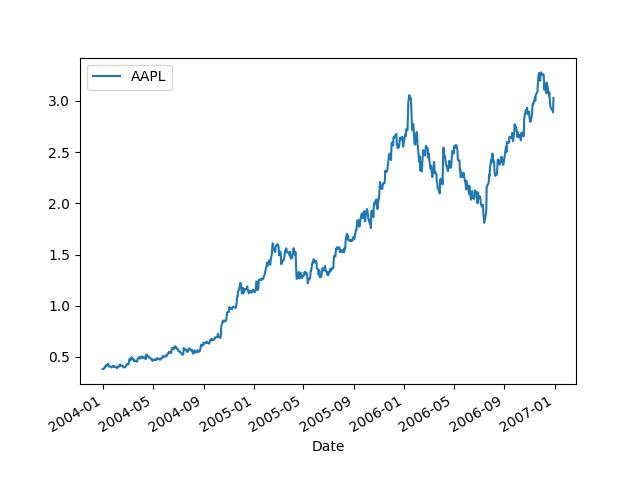
\includegraphics[width=20em]{tser_011_sign_01.jpg}

Diyelim ki müneccim bir yatırımcı bu senedi ne zaman alıp, satacağını bir
şekilde biliyor. 2005-06 civarındaki çıkış öncesi alıyor, o çıkışın tepesinde
satıyor, sonra 2006-09'da tekrar geliyor, ve son düşüş öncesi yine çıkıyor.  Bu
arkadaşın alım / satım stratejisini 1 ve 0 sinyalleri ile temsil edebiliriz.

\begin{minted}[fontsize=\footnotesize]{python}
df['signal'] = 0
filt1 = (df.index > '2005-06-01') & (df.index < '2006-02-01')
df.loc[filt1,'signal'] = 1
filt2 = (df.index > '2006-09-01') & (df.index < '2007-01-01')
df.loc[filt2,'signal'] = 1
\end{minted}

Stratejinin başarısı ne olur acaba? Üstte gördüğümüz yöntemler ile hesaplayalım,

\begin{minted}[fontsize=\footnotesize]{python}
df['ret'] = df.AAPL.pct_change()
cumret = np.cumprod(1+(df.ret*df.signal))
print (cumret.tail(4))
\end{minted}

\begin{verbatim}
Date
2006-12-26    2.233475
2006-12-27    2.233750
2006-12-28    2.215938
2006-12-29    2.324721
dtype: float64
\end{verbatim}

Tüm kümülatif seriye aslında ihtiyaç yok, son gelinen getiri noktası için,

\begin{minted}[fontsize=\footnotesize]{python}
np.prod(1+(df.ret*df.signal))
\end{minted}

\begin{verbatim}
Out[1]: 2.3247214450625857
\end{verbatim}

Yüzde 232 gibi bir artış var! Bu stratejiyi yıllık kazanca nasıl çeviririz?
Stratejinin uygulandığı tüm zaman dilimlerini alırız, ve getiriyi bir sene, yani
252 zaman dilimi (yıl içindeki iş günü miktarı), için ölçekleriz. Mesela eğer 50
gün için bir getiri $g$ hesaplamışsak, bu getiriyi yukarı ölçekleyip kabaca
$g^5$ ile yıllık getiriyi hesaplayabiliriz / tüm sene bazına yukarı
ölçekleyebiliriz (çünkü $252/5 \approx 5$), sonra tüm sonuçtan bir çıkartırız
daha önce eklenen 1 etkisini iptal etmek için. Eğer eldeki zaman serisi miktarı
252'den fazla ise alta ölçekleme de yapılabilirdi, $g^{1/2}$, $g^{1/5}$ gibi,
ama bu hesaplar da yine matematiksel olarak doğrudur ve aynı yöntemle
hesaplanır. Elde edilecek olan yıllık yüzde oranı (annual percentage rate), APR,

\begin{minted}[fontsize=\footnotesize]{python}
print ('APR', ((np.prod(1.+df.ret*df.signal))**(252./len(df.ret)))-1)
\end{minted}

\begin{verbatim}
APR 0.32471861974412564
\end{verbatim}

Getiri yıllık yüzde 32.47.

Eğer strateji üstteki kadar iyi olmasaydı, mesela yatırımcı 2005-06'da
alım yapmış ama senette kalmış, sona kadar satmamış olsaydı, bu durumda,

\begin{minted}[fontsize=\footnotesize]{python}
df = pd.read_csv('../tser_008_data/AAPL.csv',index_col='Date',parse_dates=True)
df['signal'] = 0
filt1 = (df.index > '2005-06-01')
df.loc[filt1,'signal'] = 1
df['ret'] = df.AAPL.pct_change()
print (np.prod(1+(df.ret*df.signal)))
print ('APR', ((np.prod(1.+df.ret*df.signal))**(252./len(df.ret)))-1)
\end{minted}

\begin{verbatim}
2.105210500206348
APR 0.2816374105511763
\end{verbatim}

Daha düşük bir getiri elde etmiş olacaktı.

Not: Getiriyi ölçeklerken \verb!len(df.ret)! ile yukarıdaki grafiğin tümünü
kullandık fakat düşünürsek aslında bu strateji 2004-01 noktasında değil 2005-06
noktasında başlıyor. Bu sebeple tüm seri aslında daha kısa ve APR bu sebeple
daha yüksek olurdu. Neyse örneği basit tutma amacıyla bu değişikliği yapmıyoruz.

Sinyaller

Varlığı almış olmanın 1, olmamanın 0 sinyali ile belirtildiğinden
bahsettik. Aslında sinyal bazlı strateji hesabı sadece bu iki rakamla sınırlı
değildir, mesela eksi değer kullanırsak, -1 gibi, bu açığa satış stratejisini
kodlayabilirdi. Açığa satışta düşüşten kazanıldığı için zaman serisinin getiri
yüzdesi eksi 1 ile çarpılacaktır. Düşüş var ise o değer eksi değerdir ve eksi
yüzde çarpı eksi 1 artı değer olacağı için, o değişim kazanç olarak portföye
yansımış olacaktır. Değişim -0.01 olabilir, fakat o noktada strateji açığa sat,
-1 diyor ise, -1 * -0.01 = 0.01, bu sayı kazanç sayılır.

Sinyaller birden fazla varlığı da kapsayabilir, 0 ile 1 arası birkaç değer
kullanırsak (ki bu değerlerin toplamı 1 olmalıdır) o zaman sinyaller portföydeki
``dağılımı'' temsil edebilir. Sinyal 1 sonuçta bir zaman aralığındaki tüm
değişimden istifade etmek demektir, eğer mesela 0.5 ile çarparsam değişimin
sadece yarısından istifade ediyorum, paranın yarısının o varlığa koymuşum, diğer
yarısı 0.5 ile başka bir değişimi çarpabilir, onun kazancı (ya da kaybı)
kümülatife yansır.

Alttaki örnekle devam edelim, iki tane zaman serisi görüyoruz, önce onların
yüzde değişimlerini hesaplıyoruz,

\begin{minted}[fontsize=\footnotesize]{python}
import pandas as pd

a = np.array([2.0, 2.03, 2.07, 2.11, 2.13, 2.17, 2.25, 2.29, 2.33, 2.4])
b = np.array([4.0, 4.06, 4.11, 4.17, 4.22, 4.28, 4.33, 4.39, 4.44, 4.5])

a = pd.Series(a); b = pd.Series(b)
print (list(np.round(a.pct_change(),2)))
print (list(np.round(b.pct_change(),2)))
\end{minted}

\begin{verbatim}
[nan, 0.01, 0.02, 0.02, 0.01, 0.02, 0.04, 0.02, 0.02, 0.03]
[nan, 0.01, 0.01, 0.01, 0.01, 0.01, 0.01, 0.01, 0.01, 0.01]
\end{verbatim}

Bariz şekilde birinci seri ikinciye göre daha çok yükseliyor. Bu seriler
üzerinde yarı yarıya dağılım yaparsak elde edilecek kazancı hesaplayalım
şimdi. \verb!DataFrame! yaratılır,

\begin{minted}[fontsize=\footnotesize]{python}
df = pd.concat([a,b],axis=1)
df.columns = ['a','b']
print (df)
print (df.shape)
\end{minted}

\begin{verbatim}
      a     b
0  2.00  4.00
1  2.03  4.06
2  2.07  4.11
3  2.11  4.17
4  2.13  4.22
5  2.17  4.28
6  2.25  4.33
7  2.29  4.39
8  2.33  4.44
9  2.40  4.50
(10, 2)
\end{verbatim}

Veri \verb!(10,2)! boyutlarında, iki varlığın fiyat seviyelerini gösteren 10
zaman dilimi var. Şimdi sinyali ikiye bölüyoruz, biri varlık a diğeri b için,
dağılım 0.5, 0.5 olacak, bu dağılımı 10 kere tekrarlayacağız, getirilerin
matrisini bu dağılım matrisi ile çarpacağız, sonucu toplayacağız.  Sonuçta
elimize aynen tek varlık durumunda olduğu gibi tek boyutlu bir getiri zaman
serisi geçecek.

Not: Dağılım her zaman diliminde aynı, o zaman niye (10,2) boyutlu bir matris
kullandık? Burada göstermiyoruz ama dağılımlar da zamana göre değişebilir,
dinamik karakterde olabilir. Bu tür stratejileri ilerideki derslerde göreceğiz.

\begin{minted}[fontsize=\footnotesize]{python}
positions = np.zeros(df.shape)
positions[:,0] = 0.5
positions[:,1] = 0.5
ret = (df.pct_change() * positions).sum(axis=1)
print (ret)
\end{minted}

\begin{verbatim}
0    0.000000
1    0.015000
2    0.016010
3    0.016961
4    0.010735
5    0.016499
6    0.024274
7    0.015817
8    0.014428
9    0.021778
dtype: float64
\end{verbatim}

Bu serinin başarısını hesaplayalım,

\begin{minted}[fontsize=\footnotesize]{python}
print (np.prod(1+ret))
print ('APR', ((np.prod(1+ret))**(252./len(ret)))-1)
\end{minted}

\begin{verbatim}
1.1620428461381263
APR 43.01472199080321
\end{verbatim}

Eğer dağılım farklı olsaydı, 

\begin{minted}[fontsize=\footnotesize]{python}
positions = np.zeros(df.shape)
positions[:,0] = 0.8
positions[:,1] = 0.2
ret = (df.pct_change() * positions).sum(axis=1)
print (np.prod(1+ret))
print ('APR', ((np.prod(1+ret))**(252./len(ret)))-1)
\end{minted}

\begin{verbatim}
1.1847063822264405
APR 70.61274939993416
\end{verbatim}

Bu sonuç mantıklı çünkü varlık a daha hızlı artıyordu, ağırlığı oraya daha fazla
veren strateji tabii ki daha iyi kazandırır.

Akla gelebilecek sorular, eğer bir seri diğerinden daha iyi getiri veriyorsa
niye hep ona, hatta sadece ona ağırlık verilmez? Cevabın ilk kısmı üstteki
yapılan test geriye dönük bir test olduğu, geriye dönük test ileri fiyatların
garantisi olmaması. Ayrıca veri uyduruk, gerçek dünya şartlarında iki serinin
birbirini dengeleyici bazı özellikleri olabilir, mesela genellikle birleşik
performansı ortalama olsa da iki seriden birinin sert düşüşünü diğerinin
dengeleyici özelliği varsa, portföyün getirisi uzun vadede daha sağlam
olabilir.

Birleşik portföy avantajını iyi gösteren bir örnek 60/40 kuralı, yatırımcılıkta
bilinen ünlü bir dağılım yatırımın yüzde 60'inin senet yüzde 40'inin tahvil
olması tavsiyesidir. Acaba bu dağılım hakikaten işliyor mu? Geri dönük testlerle
kontrol edebiliriz. 

Veri SP 500 indisini baz alan \verb!SPY! ve tahvilleri baz alan \verb!AGG! fon
fiyatları olacak [2,3]. Bu iki zaman serisini genel bir borsa, ve tahvil fiyatı
yerine kullanacağız. Farklı karışım oranları deneyeceğiz, ve her dağılım için
getiri performansını hesaplayacağız.

\begin{minted}[fontsize=\footnotesize]{python}
import pandas as pd
df = pd.read_csv('eqbnd.csv',index_col='Date',parse_dates=True)
df = df[(df.index > '2003-01-01') & (df.index < '2010-01-01')]
positions = np.zeros(df.shape)
print ('Senet  Tahvil')
for x in np.linspace(0,1,11):
   x = np.round(x,4)
   positions[:,0] = x
   positions[:,1] = 1.0-x
   ret = (df.pct_change() * positions).sum(axis=1)
   print ('%0.3f   %0.3f   %0.3f' % (x, np.round(1-x,2), np.round(np.prod(1.0+ret),3)))
\end{minted}

\begin{verbatim}
Senet  Tahvil
0.000   1.000   1.318
0.100   0.900   1.347
0.200   0.800   1.373
0.300   0.700   1.394
0.400   0.600   1.410
0.500   0.500   1.421
0.600   0.400   1.427
0.700   0.300   1.429
0.800   0.200   1.425
0.900   0.100   1.416
1.000   0.000   1.402
\end{verbatim}

Sonuca göre 60/40 iyi gözüküyor, gerçi 70/30 en iyisi. Demek ki bahsedilen
dağılımın iyi performans verdiği doğruymuş. Ayrıca dikkat edersek bahsedilen
oran her iki varlığın tek başına olan performansından daha iyi.

\begin{minted}[fontsize=\footnotesize]{python}
ret = ge_df.SPY.pct_change()
print ('Senet',np.round(np.prod(1.0+ret),2))
ret = ge_df.AGG.pct_change()
print ('Tahvil',np.round(np.prod(1.0+ret),2))
\end{minted}

\begin{verbatim}
Senet 1.4
Tahvil 1.32
\end{verbatim}

Not: Üstteki hesap her şartta işleyen yatırım tavsiyesi olarak alınmasın, 60/40
kuralının artık işlemediği de söyleniyor, ayrıca her ülke piyasası diğerine
benzemeyebilir. Her strateji işletilmede önce güncel veri ile test edilmelidir.

Kaynaklar

[1] \url{https://www.quantstart.com/qstrader/tutorial-60-40-portfolio/}

[2] \url{https://finance.yahoo.com/quote/SPY/}

[3] \url{https://finance.yahoo.com/quote/AGG/}
  
\end{document}
